\documentclass[output=paper]{langsci/langscibook} 
\ChapterDOI{10.5281/zenodo.2579047}

\usepackage{commands}

\title{Multilingual parsing and {M}{W}{E} detection} 
\author{Vasiliki Foufi\affiliation{University of Geneva}\and Luka Nerima\affiliation{University of Geneva}\lastand Eric Wehrli\affiliation{University of Geneva}}

%\epigram{}

\abstract{Identifying multiword expressions (MWEs) in a sentence in order to ensure their proper processing in subsequent applications, like machine translation, and performing the syntactic analysis of the sentence are interrelated processes. In our approach, priority is given to parsing alternatives involving collocations, and hence collocational information helps the parser through the maze of alternatives, with the aim to lead to substantial improvements in the performance of both tasks (collocation identification and parsing), and in that of a subsequent task (machine translation).}

\begin{document}
\maketitle

\section{Introduction}

Multiword expressions (MWEs) are lexical units consisting of more than one word (in the intuitive sense of \textit{word}). There are several types of MWEs, including \isi{idioms} (\textit{a frog in the throat}, \textit{break a leg}), fixed phrases (\textit{per se}, \textit{by and large}, \textit{rock'n roll}), noun compounds (\textit{traffic lights}, \textit{cable car}), \isi{phrasal verbs} (\textit{look up}, \textit{take off}), etc. While easily mastered by native speakers, their detection and/or their interpretation pose a major challenge for computational systems, due in part to their flexible and heterogeneous nature. 

In our research, MWEs are categorized in five subclasses: compounds, discontinuous words, named entities, collocations and \isi{idioms}. While the first three are expressions of lexical categories (N, V, Adj, etc.) and can therefore be listed along with simple words, collocations and \isi{idioms} are expressions of phrasal categories (NPs, VPs, etc.). The identification of compounds and named entities can be achieved during the lexical analysis, but the identification of discontinuous words (e.g., particle verbs or \isi{phrasal verbs}), collocations and \isi{idioms} requires grammatical data and should be viewed as part of the parsing process. 

In this chapter, we will primarily focus on collocations, roughly defined as arbitrary and conventional associations of two words (not counting grammatical words) in a particular grammatical configuration (adjective-noun, noun-noun, verb-object, etc.). Throughout this chapter, we will refer to words belonging to such associations as \textsc{content words}. We will
argue that the identification of collocations and parsing are interrelated processes -- in the sense that one cannot precede the other --  and we will show how this has been achieved in the Fips \isi{multilingual parser} \citep{wehrli07,wn15}.%(Wehrli 2007, Wehrli \& Nerima 2015). 

Section~\ref{fou:sec2} will give a brief review of MWEs and previous work. Section~\ref{fou:sec3} will describe how Fips handles MWEs and the way they are represented in our lexical database. Section~\ref{fou:sec4} will be concerned with the treatment of collocation types which present a fair amount of syntactic \isi{flexibility} (e.g. verb-object). For instance, verbal collocations may undergo syntactic processes such as \isi{passivization}, \isi{relativization}, interrogation and even \isi{pronominalization}, which can leave the collocation constituents far away from each other and/or reverse their canonical order. Section~\ref{fou:sec5} will present the collocation extraction process, which will be evaluated in Section~\ref{fou:sec6}. Finally we will conclude in Section~\ref{fou:sec7}.


\section{Multiword expressions: A brief review of related work}
\label{fou:sec2}
The standard approach in dealing with MWEs in parsing is to apply a ``words-with-spaces'' preprocessing step, which marks the MWEs in the input sentence as units which will later be integrated as single blocks in the parse tree built during analysis \citep{brun:1998,zhang06}. This method is not really adequate for processing collocations. Unlike other expressions that are fixed or semi-fixed, several collocation types do not allow a ``words-with-spaces'' treatment because they have a high morphosyntactic \isi{flexibility}.
On the other hand, \cite{alegria04} and \cite{villavicencio07} adopted a compositional approach to the encoding of MWEs, able to capture more morphosyntactically flexible MWEs. \cite{alegria04} showed that by using a MWE processor in the preprocessing stage, a significant improvement in the POS tagging precision is obtained. \cite{villavicencio07} found that the addition of 21 new MWEs to the lexicon led to a significant increase in the \isi{grammar} coverage (from 7.1\% to 22.7\%), without altering the \isi{grammar} accuracy.
However, as argued by many researchers (e.g., \citealt{heid94,seretan11}), \isi{collocation identification} is best performed on the basis of parsed material. This is due to the fact that collocations are co-occurrences of lexical items in a specific syntactic configuration. For that reason, we have chosen the identification of collocations as soon as possible during parsing. 
\cite{finkeljr09} have built a joint model of parsing and named entity recognition, based on a discriminative feature-based constituency parser. They tested their model on the OntoNotes annotated corpus\footnote{\url{http://www.gabormelli.com/RKB/OntoNotes_Corpus}, last accessed 26 February 2019.} and they achieved a remarkably good performance on both parsing and recognition of named entities. \cite{green13} have developed two structured prediction models with the aim to identify arbitrary-length, contiguous MWEs in \ili{Arabic} and \ili{French}. The first is based on context-free grammars and the second uses tree substitution grammars, a formalism that can store larger syntactic fragments. They claim that these techniques can be applied to any language for which a syntactic treebank, a MWE list, and a morphological analyzer exist. \cite{nasretal15} have developed a joint parsing and MWE identification model for the detection and representation of ambiguous complex function words. \cite{constantnivre16} developed a transition-based parser which combines two factorized substructures: a standard tree representing the syntactic dependencies between the lexical elements of a sentence and a forest of lexical trees including MWEs identified in the sentence. 


\section{The Fips parser}
\label{fou:sec3}
Fips is a \isi{multilingual parser}, available for several languages, i.e. \ili{French}, \ili{English}, \ili{German}, \ili{Italian}, \ili{Spanish}, \ili{Modern Greek}, \ili{Romanian} and Portuguese. It relies on generative \isi{grammar} concepts and is basically made up of a generic parsing module which can be refined in order to suit the specific needs of a particular language. Fips is a constituent parser that functions as follows: it scans an input string from left to right, without any backtracking. The parsing algorithm, iteratively, performs the following three steps:
%%\renewcommand{\labelitemi}{$\bullet$}
\begin{itemize}
\item get the next lexical item and project the relevant phrasal category\\ (X $\rightarrow$ XP);
\item merge XP with the structure in its left context (the structure already built);
\item (syntactically) interpret XP, triggering procedures 
	\begin{itemize}
		\item to build predicate-argument structures
		\item to create  chains linking preposed elements to their trace
		\item to find the antecedent of (3rd person) personal pronouns
		\item to identify collocations. 
	\end{itemize}
\end{itemize}
 
The parsing procedure is a one-pass (no pre-processing, no post-processing) scan of the input text, using rules to build up constituent structures and (syntactic) interpretation procedures to determine the dependency relations between constituents (grammatical functions, etc.), including cases of \isi{long-distance dependencies}.
One of the key components of the parser is its lexicon, which contains detailed morphosyntactic and semantic information, selectional properties, valency information, and syntactico-semantic features that are likely to influence the syntactic analysis. 

\subsection{The Fips lexicon}

The lexicon was built manually and contains fine-grained information required by the parser. It is organized as a relational database with four main tables:

\begin{description}
\item[words,] representing all morphological forms (spellings) of the words of a language, grouped into inflectional paradigms; 
\item[lexemes,] describing more abstract lexical forms which correspond to the syntactic and semantic readings of a word (a lexeme corresponds roughly to a standard dictionary entry); 
\item[collocations,] which describe multiword expressions combining two lexical items, not counting function words;
\item[variants,] which list all the alternatives written forms for a word, e.g. the written forms of British \ili{English} vs American \ili{English}, the spellings introduced by a spelling reform, presence of both literary and modern forms in Greek, etc.
\end{description}

\subsection{Representation of MWEs in the lexicon}

In the introduction we mentioned that in our research, MWEs are categorized in five subclasses, i.e. compounds, discontinuous words, named entities, collocations and \isi{idioms}.
We will now describe how they are represented in the lexical database.

Compounds and named entities are represented by the same structure as simple words. An entry describes the syntactic and (some) semantic properties of the word: lexical category (POS),
type (e.g., common noun, auxiliary verb), subtype, selectional features, argument structure, semantic features, thematic roles, etc. Each entry is associated with the inflectional paradigm of the word, 
that is all the inflected forms of the word along with the morphological features (number, gender, person, case, etc.). The possible spaces or hyphens of the compounds are processed 
at the lexical analyzer level in order to distinguish those that are separators from those belonging to the compound.

Discontinuous words, such as particle verbs or \isi{phrasal verbs}, are represented in the same way as simple words as well, except that the orthographic string contains the bare verb only, 
the particle being represented separately in a specific field. The benefit of such an approach is that the phrasal verb inherits the inflectional paradigm of the basic verb. For agglutination,
a lexical analyzer will detect and separate the particle from the basic verb.

%Named entities are represented as simple word too. They have some specificities: they are proper nouns and as such they have only one or a few morphological forms. They usually have an abbreviation represented as an alternative written from, stored in the table of variants.

Collocations are defined as associations of two lexical units (not counting function words) in a specific syntactic relation (for instance adjective-noun, verb-object, etc.). 
A lexical unit can be a word or a collocation. The definition is therefore recursive and enables to encode collocations that have more than two words \citep{nws10}. 
For instance, the \ili{French} collocation \textit{tomber en panne d’es\-sence} (`to run out of gas') is composed of the word \textit{tomber} (lit. `fall') and the collocation \textit{panne d'essence} (lit. `failure of gas'). Similarly, the \ili{English} collocation 
\textit{guaranteed minimum wage} is composed of the word \textit{guaranteed} and the collocation \textit{minimum wage}.

In addition to the two lexical units, a collocation entry encodes the following information: 
the citation form, the collocation type (i.e., the syntactic relation between its two components), the preposition (if any) and a set of syntactic frozenness constraints. 

Some examples of  entries are given in (\ref{fou:lex1}), (\ref{fou:lex2}) and (\ref{fou:lex3}). %Figure~\ref{fou:figex}.

%\begin{figure}[htbp]
%  \hspace*{3mm}\parbox{10cm}{

\begin{exe}
  %\makeex{
  \ex\label{fou:lex1}
           {\em ein Schlaglicht werfen } (DE) `to highlight' \\
           type : verb-direct object \\
           lexeme \#1 : {\em Schlaglicht} `spotlight', noun-noun collocation\\
           lexeme  \#2: {\em werfen} `throw', \_ NP PP verb\\
           preposition : $\emptyset$ \\
           features : \{\}
  %}
%}
  
%\clearpage

%\vspace*{2mm}

%\hspace*{3mm}\parbox{10cm}{

  %\makeex{
  \ex\label{fou:lex2}
           {\em  κινητό τηλέφωνο} (kinitó tiléfono) (MG) `mobile phone' \\
           type : adjective-noun \\
           lexeme  \#1 : {\em κινητό} (kinitó) `mobile', adjective\\
           lexeme  \#2 : {\em τηλέφωνο} (tiléfono) `phone', noun \\
           preposition : $\emptyset$ \\
           features : \{\}
  %}
%}
  
%\vspace*{2mm}

%\hspace*{3mm}\parbox{10cm}{

%\makeex{
  \ex\label{fou:lex3}
           {\em banc de poissons} (FR) `shoal of fish' \\
           type : noun-prep-noun \\
           lexeme  \#1 : {\em banc} `bench', noun \\
           lexeme  \#2 : {\em poisson} `fish', noun \\
           preposition :  {\em de} `of'\\
           features : \{determiner-less complement, plural complement\}
   %}
%}
\end{exe}           

%\vspace*{2mm}
%\caption{\label{fou:figex} Multiword lexical entries}
%\end{figure}

For the time being, we represent \isi{idioms} as collocations with more restriction features (cannot passivize, no modifiers, etc.). They are, therefore, stored in the same database table. Reducing \isi{idioms} to collocations with specific features though convenient and appropriate for large classes of \isi{idioms} is nevertheless not general enough. In particular, it does not allow for the representation of \isi{idioms} with fixed phrases, such as \textit{to get a foot in the door}. 



\subsection{Fips and collocations}
\subsubsection{Collocation identification mechanism}
\label{fou:ref:subsubsec:colidme}
The \isi{collocation identification} mechanism is integrated in the parser. In the pre\-sent version of Fips, collocations, if present in the lexicon, are identified in the input sentence during the analysis of that sentence, rather than at the end. In this way, priority is given to parsing alternatives involving collocations, and collocational information helps the parser through the maze of alternatives. 
To fulfill the goal of interconnecting the parsing procedure and the identification of collocations, we have incorporated the \isi{collocation identification} mechanism within the constituent attachment procedure (see next section)\todo{Do you mean Sect 3.3.2 or Sect. 4?}. The Fips parser, like many grammar-based parsers, uses left attachment and right attachment rules to build respectively left subconstituents and right subconstituents. The \isi{grammar} used for the computational modelling comprises rules and procedures. Attachment rules describe the conditions under which constituents can combine, while procedures compute properties such as \isi{long-distance dependencies}, agreement, control properties, argument-structure building, and so on. 

\subsubsection{Treatment of collocations}

The identification of compounds and named entities can be achieved during the lexical analysis, but the identification of discontinuous words, collocations and \isi{idioms} requires grammatical data and are, therefore, part of the parsing process. The identification of a collocation occurs when the second lexical unit of the collocation is attached, either by means of a left attachment rule (e.g., adjective-noun, noun-noun) or by means of a right-attachment rule (e.g., noun-adjective, noun-prep-noun, verb-object), as shown in example~(\ref{fou:exFirst}). %(\refex{1}) and Figure~\ref{fou:exFirst}.

%% \makeex{Paul took up a new challenge. 
%% }

%% \begin{figure}
%%   \noindent
%%   {\small
%%     \cat{TP}{\cat{DP}{Paul}\cat{VP}{took up \cat{DP}{a \cat{NP}{\cat{AP}{new} challenge}}}}
%%   }
%%   \caption{\label{fou:exFirst} Parse structure for sentence `Paul took up a new challenge'}
%% \end{figure}

%% 
\begin{exe}
  \ex\label{fou:exFirst}
  Paul took up a new challenge.\\
  {\small \cat{TP}{\cat{DP}{Paul}\cat{VP}{took up \cat{DP}{a \cat{NP}{\cat{AP}{new} challenge}}}} }
\end{exe}

When the parser reads the noun \textit{challenge} and attaches it (along with the prenominal adjective) as complement of the incomplete  \cat{DP}{a} direct object of the verb \textit{take up}, the identification procedure considers iteratively all the governing nodes of the attached noun and checks whether the association of the lexical head of the governing node and the attached element constitutes an entry in the collocation database. The process stops at the first governing node of a major category (noun, verb or adjective). In our example, going up from \textit{challenge}, the process stops at the verb \textit{take up}. Since \textit{take up - challenge} is an entry in the collocation database and its type (verb-object) corresponds to the syntactic configuration, the identification process succeeds.

In several cases the two constituents of a collocation can be very far apart, or do not appear in the expected order. We will turn to such examples in Section~\ref{fou:sec4}. To handle them, the identification procedure sketched above must be slightly modified so that not only the attachment of a lexical item triggers the identification process, but also the attachment of the trace of a preposed lexical item. In such a case, the search will consider the antecedent of the trace. 
This shows, again, that the main advantage provided by a syntactic parser in such a task is its ability to identify collocations even when complex grammatical processes disturb the canonical order of constituents.


\section{Detection of collocations in free word-order languages}
\label{fou:sec4}
Just as other types of MWEs, collocations are problematic for NLP because they have to be recognized and treated as a whole, rather than compositionally \citep{sag02}. On the other hand, there is no systematic restriction on lexical forms which constitute a collocation, on the order of items in a collocation, or on the number of words that may intervene between these items especially in \isi{free word-order} languages. In such languages, the direct object of a \isi{verbal collocation} can be found either before or after the verb, with or without intervening material. This is illustrated in the following examples with the Greek verb-object collocation {\em κάνω έκκληση} (káno éklisi)
`to make an appeal'. 
In (\ref{fou:exMinister}a), %(\refex{1})a,
the direct object 
%(in bold face) 
follows the verb, while in (\ref{fou:exMinister}b), %(\refex{1})b,
it precedes the verb, with several intervening words between them:

%% %% \debex{%% Ο Υπουργός Παιδείας \textbf{έκανε έκκληση} στους διοικητικούς υπαλλήλους να σταμα\-τήσουν την απεργία. \\ 
%% %% Ο Ιpurgós Pedías \textbf{ékane éklisi} stus diikitikús ipalílus ná stamatísun tín aperyía\\
%% %% `The Minister of Education \textbf{made an appeal} to the administrative staff to stop the strike.'
%% {\gll Ο Υπουργός Παιδείας \textbf{έκανε έκκληση} στους διοικητικούς υπαλλήλους να σταμα\-τήσουν την απεργία. \\
%% Ο Ιpurgós Pedías \textbf{ékane éklisi} stus diikitikús ipalílus ná stamatísun tín aperyía\\
%% \glt `The Minister of Education \textbf{made an appeal} to the administrative staff to stop the strike.'}
%% }

%% \putex{%% \textbf{Έκκληση} στους διοικητικούς υπαλλήλους να σταματήσουν την απεργία \textbf{έκανε} ο Υπουργός Παιδείας.} \\ 
%% %% \textbf{Éklisi} stus diikitikús ipalílus ná stamatísun tín aperyía \textbf{ékane} o Ιpurgós Pedías\\
%% %% `\textbf{An appeal} to the administrative staff to stop the strike \textbf{made} the Minister of Education.'
%% {\gll \textbf{Έκκληση} στους διοικητικούς υπαλλήλους να σταματήσουν την απεργία \textbf{έκανε} ο Υπουργός Παιδείας. \\
%% \textbf{Éklisi} stus diikitikús ipalílus ná stamatísun tín aperyía \textbf{ékane} o Ιpurgós Pedías\\
%% \glt `\textbf{An appeal} to the administrative staff to stop the strike \textbf{made} the Minister of Education.'}
%% }
%% \finex

\eal\label{fou:exMinister}
\ex[]{
  \gll Ο Υπουργός Παιδείας \textit{έκανε έκκληση} στους διοικητικούς υπαλλήλους να σταμα\-τήσουν την απεργία. \\
  Ο Ιpurgós Pedías \textit{ékane éklisi} stus diikitikús ipalílus ná stamatísun tín aperyía\\
  \glt ‘The Minister of Education \textit{made an appeal} to the administrative staff to stop the strike.’
}
\ex[]{
  \gll \textit{Έκκληση} στους διοικητικούς υπαλλήλους να σταματήσουν την απεργία \textit{έκανε} ο Υπουργός Παιδείας. \\
  \textit{Éklisi} stus diikitikús ipalílus ná stamatísun tín aperyía \textit{ékane} o Ιpurgós Pedías\\
  \glt ‘\textit{An appeal} to the administrative staff to stop the strike \textit{made} the Minister of Education.’
}
\zl

\subsection{ Nominal collocations}
Modifiers can often be attached within a \isi{nominal collocation}, separating the two terms. For example, between the constituents of a \isi{nominal collocation} in the form of adjective-noun, other lexemes may interfere. Table~\ref{fou:fig1} shows a part of the analysis of a sentence where the possessive determiner \textit{του} (tu) `his' occurs between the adjective  \textit{παρθενικό} (parthenikό) `maiden' and the noun \textit{ταξίδι} (taxίdi) `voyage' of the collocation \textit{παρθενικό ταξίδι} (parthenikό taxίdi) `maiden voyage'. Note that, for the POS tagset, we opted for the universal tagset \citep{petrov12}. 

\begin{table}[h]
  {\small
    \begin{tabular}{l>{\scshape}lrl}
      \lsptoprule
      word & \normalfont tag & position & collocation \\ %\hline
      \midrule
          \textit{Το} (to) `the'                   & det & 1\\
          \textit{παρθενικό} (parthenikό) `maiden' & adj & 4 \\
          \textit{του } (tu) `his'                 & pron & 14 \\
          \textit{ταξίδι} (taxίdi) `voyage'        & noun & 18 & \textit{παρθενικό ταξίδι} \\
          & & & `maiden voyage' \tabularnewline
          \lspbottomrule
    \end{tabular}
  }
\caption{\label{fou:fig1}Identification of the nominal collocation \textit{παρθενικό ταξίδι} (parthenikό taxίdi) `maiden voyage'}
\end{table} 


\subsection{Verbal collocations}
Verb-object collocations may undergo syntactic processes such as \isi{passivization}, \isi{relativization}, interrogation and even \isi{pronominalization}, which can leave the collocation constituents far away from each other and/or reverse their canonical order.



%\paragraph*{Passive} {~~~} \\
\subsubsection{Passive}
In passive constructions, the direct object is promoted to the subject position leaving an empty constituent in the direct object position. The detection of a verb-object collocation in a passive sentence is thus triggered by the insertion of the empty constituent in direct object position. The \isi{collocation identification} procedure checks whether the antecedent of the (empty) direct object and the verb constitute a verb-object collocation.
In example (\ref{fou:exDecision}), %(\refex{1}),
the noun  \textit{απόφαση} (apófasi) `decision' of the collocation \textit{παίρνω απόφαση} (pérno apófasi) `to make a decision'  precedes the verb and is in the nominal case, the usual case for subjects.

%% \makeex{%%  {Η απόφαση πάρθηκε.} \\ I apófasi párthike \\
%%   %% `The decision was made.'
%% {\gll Η απόφαση πάρθηκε. \\
%% I apófasi párthike. \\
%% \glt `The decision was made.'}
%% }
\ea\label{fou:exDecision}
\gll Η απόφαση πάρθηκε. \\
I apófasi párthike. \\
\glt `The decision was made.'
\z

%\paragraph*{Pronominalization}  {~~~} \\
\subsubsection{Pronominalization}
Another transformation that can affect some collocation types is \isi{pronominalization}.  In such cases, it is important to identify the antecedent of the pronoun which can be found either in the same sentence or in the context. Example (\ref{fou:exMoney}) %(\refex{1})
illustrates a \isi{phrase} where the pronoun \textit{it} refers to the noun \textit{money}. Since the pronoun is the subject of the passive form \textit{would be well spent}, it is interpreted as the direct object of the verb and therefore stands for an occurrence of the collocation \textit{to spend money}.

%% \makeex{
%%  ...though where the money would come from, and how to ensure that\textbf{ it}
%% would be well \textbf{spent}, is unclear.}
\ea\label{fou:exMoney}
  \ldots{} though where the money would come from, and how to ensure that\textit{ it}
would be well \textit{spent}, is unclear.
\z

In example (\ref{fou:exLet}) %(\refex{1})
and Table~\ref{fou:fig2}, both the verb \textit{να αναλάβουν} (na analávun) `to take' of the verb-object collocation \textit{αναλαμβάνω ευθύνη} (analamváno efthíni) `to take responsibility' and the pronominalized object \textit{τις} (tis) `them' are found in another sentence.

%% \makeex{%%
%% %% {Ας αναλογιστούν τις ευθύνες τους. 	Να τις αναλάβουν.} \\ As analogistún tis efthínes tus. Na tis analávun\\
%% %% `Let them consider their responsibilities. Should they take them.'
%% {\gll Ας αναλογιστούν τις ευθύνες τους. Να τις αναλάβουν. \\
%% As analogistún tis efthínes tus. Na tis analávun. \\
%% \glt `Let them consider their responsibilities. Should they take them.'}
%% }
\ea\label{fou:exLet}
\gll Ας αναλογιστούν τις ευθύνες τους. Να τις αναλάβουν. \\
As analogistún tis efthínes tus. Na tis analávun. \\
\glt `Let them consider their responsibilities. Should they take them.'
\z

\begin{table}[h]
  \fittable{%
    {\small
      \begin{tabular}{l>{\scshape}lrl}
        \lsptoprule
        word & \normalfont tag & position & collocation \\ %\hline
        \midrule
            \textit{Ας}	(as) `Let them'                 & prt & 1 \\		
            \textit{αναλογιστούν} (analogistún) `consider' & verb &	4	\\
            \textit{τις}	(tis) `the'                     & det &	17	\\	
            \textit{\textbf{ευθύνες}} (efthínes)  `responsibilities' &	noun &	21 \\	
            \textit{τους} (tus) `their' &	pron &	21	\\
            .  & punc & 33 \\\tablevspace

            \textit{Να}  (Na) `Should'	& conj & 35 \\		
            \textit{\textbf{τις}} (tis)	`them' & pron &	35 \\ 		
            \textit{αναλάβουν} (analávun) `take' &	verb &	42	& 	\itshape αναλαμβάνω την ευθύνη \\
            & & & `take responsibility'\\
            . &	punc &	51 \tabularnewline
            \lspbottomrule
      \end{tabular}
  }}
 \caption{\label{fou:fig2}Identification of a verbal collocation}
\end{table} 

Example (\ref{fou:exRecord}) %(\refex{1})
and Table~\ref{fou:fig3} concern \ili{French} and show again two sentences. Each one of them contains a collocation with the noun \textit{record}: \textit{établir un record} `to set up a record' in the first one,  and \textit{battre un record} `to break a record' in the second one, where the noun is pronominalized in the form of a clitic pronoun (\textit{le} `it').

%% \makeex{
%% %% Ce \textbf{record} a été \textbf{établi} l'été dernier. Paul espère \textbf{le} \textbf{battre} bientôt.\\
%% %% `This record was set up last summer. Paul hopes to break it soon.'
%% {\gll Ce \textbf{record} a été \textbf{établi} l'été dernier. Paul espère \textbf{le} \textbf{battre} bientôt.\\
%%   This record has been {set up} last summer. Paul hopes \textbf{it} \textbf{break} soon.\\
%%   \glt `This record was set up last summer. Paul hopes to break it soon.'}
%% }
\ea\label{fou:exRecord}
 \gll Ce \textit{record} a été \textit{établi} l'été dernier. Paul espère \textit{le} \textit{battre} bientôt.\\
 This record has been {set up} last summer. Paul hopes \textit{it} \textit{break} soon.\\
 \glt `This record was set up last summer. Paul hopes to break it soon.'
\z

\begin{table}[h]
  {\small 
    \begin{tabular}{>{\itshape}l>{\scshape}lr>{\itshape}l}
      \lsptoprule
      \normalfont word & \normalfont tag & position & \normalfont collocation \\ %\hline
      \midrule
      Ce     &	det &	1	\\
      record &	noun	 & 4	\\	
      a	     &  verb & 	11	\\
      été    &  verb & 	13		\\
      établi & verb	 & 17	 & 	établir un record\\
      l'     &	det & 	24	\\
      été	 & noun	 & 26		 & 	été dernier\\
      dernier & 	adj	 & 30			\\
      .	 & punc	 & 37		\\\tablevspace

      Paul & 	noun	 & 1\\
      espère & 	verb & 	6	\\
      le	 & pron & 13	\\
      battre & 	verb	 & 16	  & 	battre un record\\
      bientôt & adv	 & 23			\\
      .	 & punc & 	30			\tabularnewline
      \lspbottomrule
\end{tabular}
  }
 \caption{\label{fou:fig3}Identification of verbal collocations, one with pronominalized object}
\end{table} 


The parser detects collocations in which the nominal element has been pron\-ominalized thanks to the \isi{anaphora} resolution component incorporated in Fips \citep{wn13}. 


%\paragraph*{\textit{Wh}-constructions} {~~~} \\
\subsubsection{\textit{Wh}-constructions}\todo[inline]{\textit{Wh} in italics in heading, but in upshape in text.}
Our parser can also cope with \isi{long-distance dependencies}, such as the ones found in \isi{wh-questions}.\footnote{wh-words are interrogative (or relative) words such as \textit{who}, \textit{what}, \textit{which}, etc. For a general discussion of wh-constructions, see \citep{chomsky77}.} In sentence (\ref{fou:exWhich}) %(\refex{1})
and Table~\ref{fou:fig4}, the direct object constituent occurs at the beginning of the sentence. Again, assuming a generative \isi{grammar} analysis, we consider that such pre-posed constituents are connected to so-called canonical positions. The fronted element being a direct object, the canonical position is a post-verbal DP position immediately dominated by the VP node. The parser establishes such a link and returns the structure from~(\ref{fou:exWhich}), where [DP~e]\ik{i} stands for the empty category (the ``trace'') of the preposed constituent \textit{Ποιο ρεκόρ} (Pxó rekór) `Which record'. 

%% \makeex{%%  {Ποιο ρεκόρ θέλει να σπάσει ο Μελισσανίδης;} \\Pxó rekór théli na spási o Melisanídis\\
%%   %% `Which record does Melissanidis want to break?'}
%%   {\gll Ποιο ρεκόρ θέλει να σπάσει ο Μελισσανίδης? \\
%%     Pxó rekór théli na spási o Melisanídis\\
%%    \glt `Which record does Melissanidis want to break?'}
%% }
\ea\label{fou:exWhich}
\gll Ποιο ρεκόρ θέλει να σπάσει ο Μελισσανίδης? \\
Pxó rekór théli na spási o Melisanídis\\
{\small\cat{CP}{\cati{DP}{Ποιο ρεκόρ}{i}} \cat{TP}{θέλει}  \cat{CP}{να} \cat{TP}{σπάσει} \cat{VP}{\cati{DP}{e}{i}} \cat{DP}{ο Μελισσανίδης}}
\glt `Which record does Melissanidis want to break?'
\z

%% \begin{figure}
%%   \noindent
%%   {\small
%%     \cat{CP}{\cati{DP}{Ποιο ρεκόρ}}{i} \cat{TP}{θέλει}  \cat{CP}{να} \cat{TP}{σπάσει} \cat{VP}{\cati{DP}{e}{i}} \cat{DP}{ο Μελισσανίδης}
%%   }
%%   \caption{\label{fou:ex1b} Parse structure for sentence `Ποιο ρεκόρ θέλει να σπάσει ο Μελισσανίδης'}
%% \end{figure}

%% \vspace*{.3mm}

\begin{table}[h]
  {\small 
    \begin{tabular}{l>{\scshape}lrl}
      \lsptoprule
      word & \normalfont tag & position & collocation \\ %\hline
      \midrule
          \textit{Ποιο} (Pio) `Which' & 	det & 	1	\\
          \textit{ρεκόρ} (rekór) `record' & noun & 	6 		 \\
          \textit{θέλει}	 (théli) `wants' & verb & 	12	 \\
          \textit{να}	(na) `to' & conj & 18	 \\
          \textit{σπάσει}	(spási) `break' & verb & 	21	 & 	\textit{σπάζω το ρεκόρ} \\ & & & `break the record'\\
          \textit{ο}  (o) `the' & det & 	28	 \\
          \textit{Μελισσανίδης}	(Melisanídis) `Melisanidis' & noun  & 30	 \tabularnewline	 %\\
          %{;}	 & other &  42
          \lspbottomrule
    \end{tabular}
  }
  \caption{\label{fou:fig4}Identification of verbal collocation in a wh-question}
\end{table} 


In such cases, the \isi{collocation identification} process is triggered by the insertion of an empty constituent in the direct object position of the verb. Since the empty constituent is connected to the pre-posed constituent, such examples can be easily treated as a minor variant of the standard case described in Section~\ref{fou:ref:subsubsec:colidme}. All so-called wh-constructions are treated in a similar fashion, that is relative clause and topicalization. 

%\paragraph*{\textit{Tough}-movement constructions}  {~~~} \\
\subsubsection{\textit{Tough}-movement constructions}
In such constructions, the matrix subject is construed as the direct object of the infinitival verb governed by a \textit{tough} adjective. Following \quotecite{chomsky77} analysis of such constructions, the parser will hypothesize an abstract wh-operator in the specifier position of the infinitival clause, which is linked to the matrix subject. Like all wh-constituents, the abstract operator will itself be connected to an empty constituent later on in the analysis, giving rise to a chain connecting the subject of the main clause and the direct object position of the infinitival clause. The structure as computed by the parser is given in~(\ref{fou:ex2}), with the chain marked by the index $i$.

%% \begin{figure}
%%   \noindent
%%   {\small
%%     %\makeex{\small
%%       \cat{TP}{\cati{DP}{this record}{i} seems\cat{AP}{difficult\cat{TP}{\cati{DP}{e}{i} to\cat{VP}{break\cati{DP}{e}{i}}}}}
%%     %}
%%   }
%%   \caption{\label{fou:ex2} Parse structure for sentence `This record seems difficult to break'}
%% \end{figure}
\ea\label{fou:ex2}
{\small \cat{TP}{\cati{DP}{this record}{i} seems\cat{AP}{difficult\cat{TP}{\cati{DP}{e}{i} to\cat{VP}{break\cati{DP}{e}{i}}}}} }
\z

\subsection{Complex collocations}
As observed by \cite{heid94}, among others, collocations can involve more than two content words. Such complex expressions can be described recursively as collocations of collocations. Our identification procedure has been extended to handle such cases. For example, the Greek noun-noun collocation \textit{απεργία πείνας} (aperyía pínas) `hunger strike', which combines with the verb \textit{κάνω} (káno) `to do', yields the larger verb-object collocation \textit{κάνω απεργία πείνας} (káno aperyía pínas) `to go on hunger strike', where the object is itself a noun-noun collocation. Given the strict left-to-right processing order assumed by the parser, the system will first identify the collocation \textit{κάνω απεργία} (káno aperyía) `to go on strike' when attaching the word \textit{απεργία} (aperyía) `strike'. Then, reading the last word, \textit{πείνας} (pínas) `hunger' (here in genitive case), the parser will identify the collocation \textit{απεργία πείνας} (aperyía pínas) `hunger strike'. The search succeeds with the verb \textit{κάνω} (káno) `to do', and the collocation \textit{κάνω απεργία πείνας} (káno aperyía pínas) `to go on hunger strike' is identified.

Moreover, the Greek lexical database comprises nominal collocations formed by a simple noun and a collocation or by two collocations. For example, \textit{δύναμη πολιτικής προστασίας} (dínami politikís prostasías) `civil protection force' is for\-med by a simple noun, \textit{δύναμη} (dínami) `force', and a \isi{nominal collocation} in genitive case, \textit{πολιτικής προστασίας} (politikís prostasías) `of civil protection'. The collocation \textit{πυρηνικός σταθμός παραγωγής ενέργειας} (pirinikós stathmós para\-goyís enéryias) `nuclear power station' is formed by the collocations \textit{πυρηνικός σταθμός} (pirinikós stathmós) `nuclear station' and \textit{παραγωγής ενέργειας} (para\-goyís enéry\-ias) `of energy production'.  


\section{Collocation extraction}
\label{fou:sec5}
As already mentioned, the parser can only identify collocations that are part of its lexical database. Therefore, it is crucial to have as good a coverage of collocations as possible in the database. To help the linguist/lexicographer in the time-consuming task of inserting collocations, we have designed a collocation  extraction tool \citep{seretan11}, dubbed FipsCo. Applied to a corpus, FipsCo parses all the sentences, extracting all the pairs of lexical items which co-occur in predefined grammatical configurations (adjective-noun, noun-noun, subject-verb, verb-object, etc.). All those pairs are considered as potential collocations.

Once the corpus has been completely parsed, a statistical filter  is used to rank the potential collocations according to their degree of association. By default, we use the log-likelihood ratio measure (LLR), since it was shown to be particularly suited to language data \citep{dunning93}. In our extractor, the items of each candidate expression represent base word forms (lemmas) and they are considered in the canonical order implied by the given syntactic configuration (e.g., for a verb-object candidate, the object is postverbal in subject-verb-object (SVO) languages like Greek). Even if the candidate occurs in corpus in different morphosyntactic realizations, its various occurrences are successfully identified as instances of the same type thanks to the syntactic analysis performed by the parser. 


\begin{figure}[p]
%\vspace*{-2cm}
%\includegraphics[scale=1, clip=true, trim=0mm 20mm 20mm 20mm] {screenshot.pdf}
  %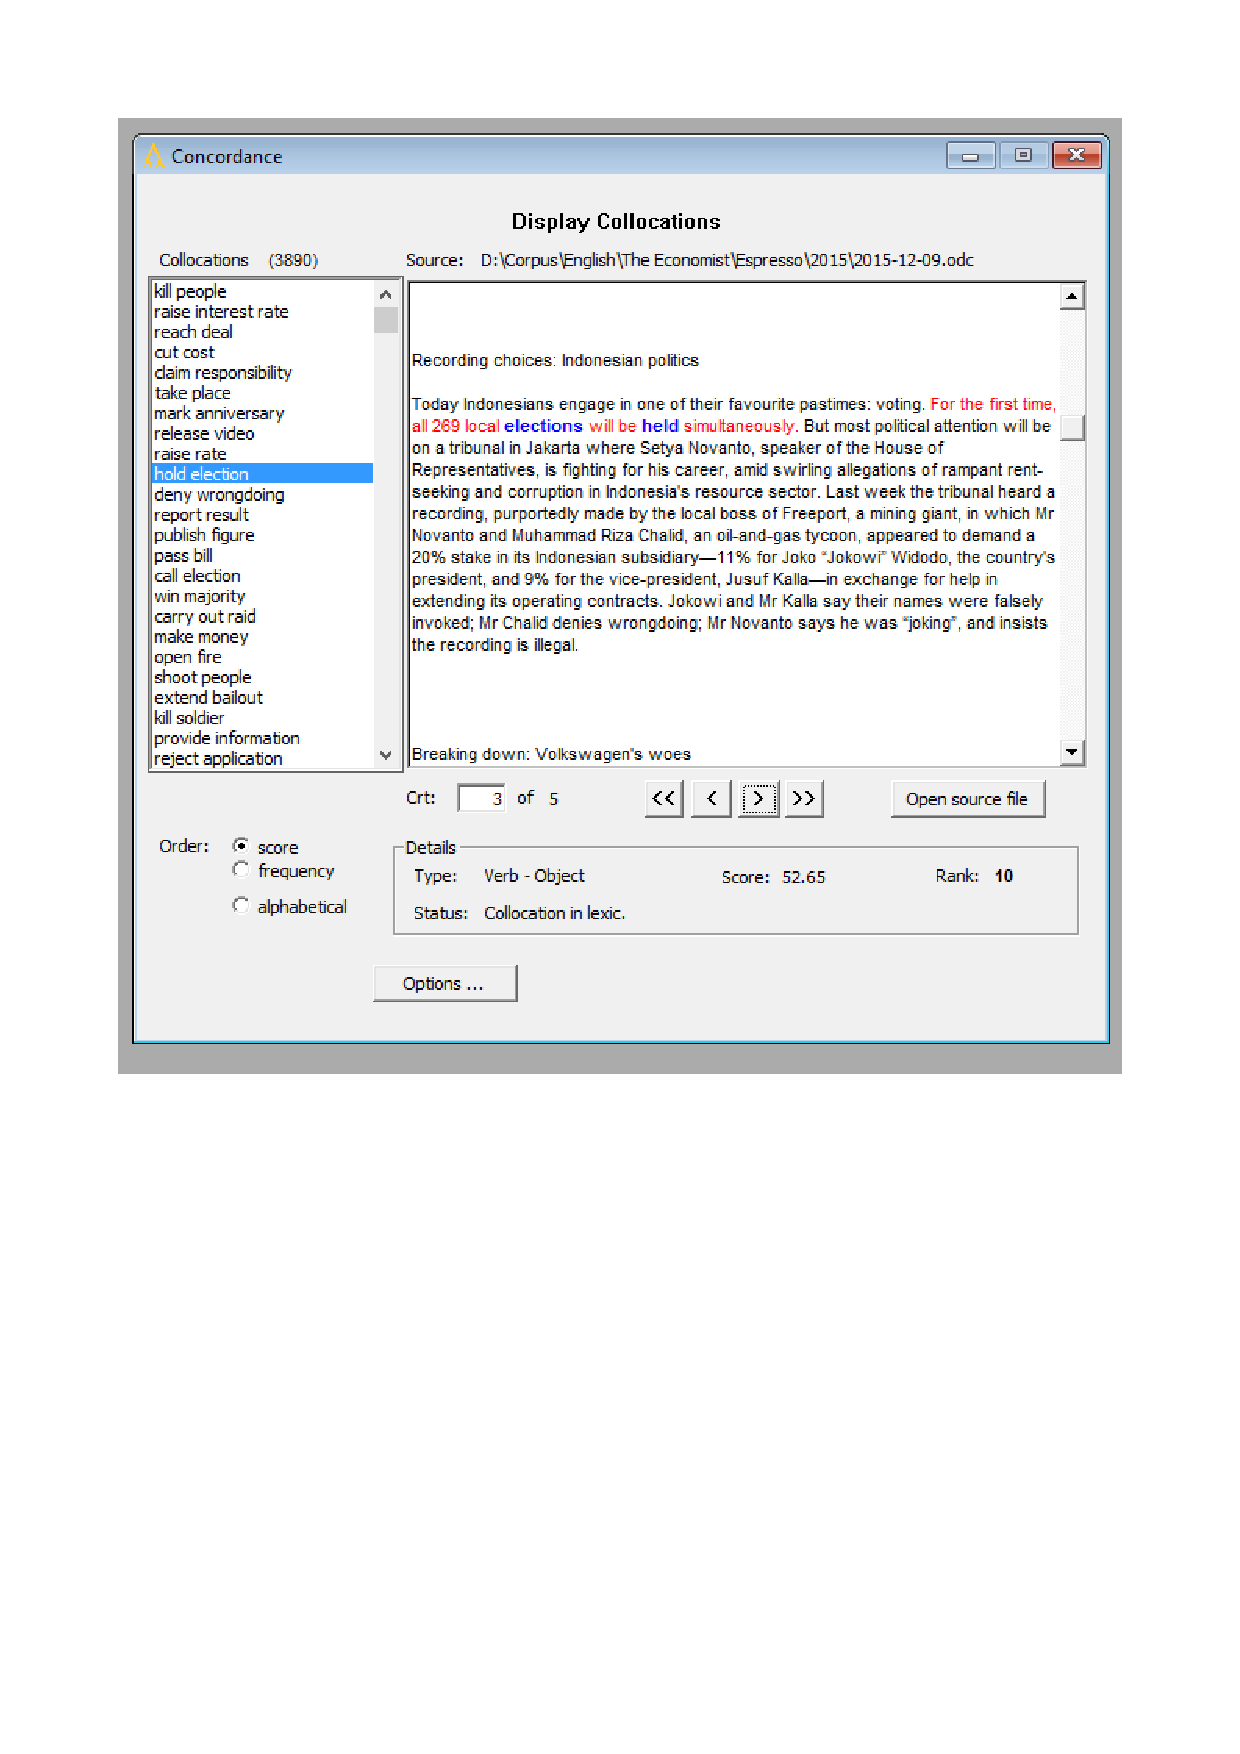
\includegraphics[scale=0.8, clip=true, trim=0mm 110mm 20mm 10mm] {figures/FipsCoPict.pdf}
%   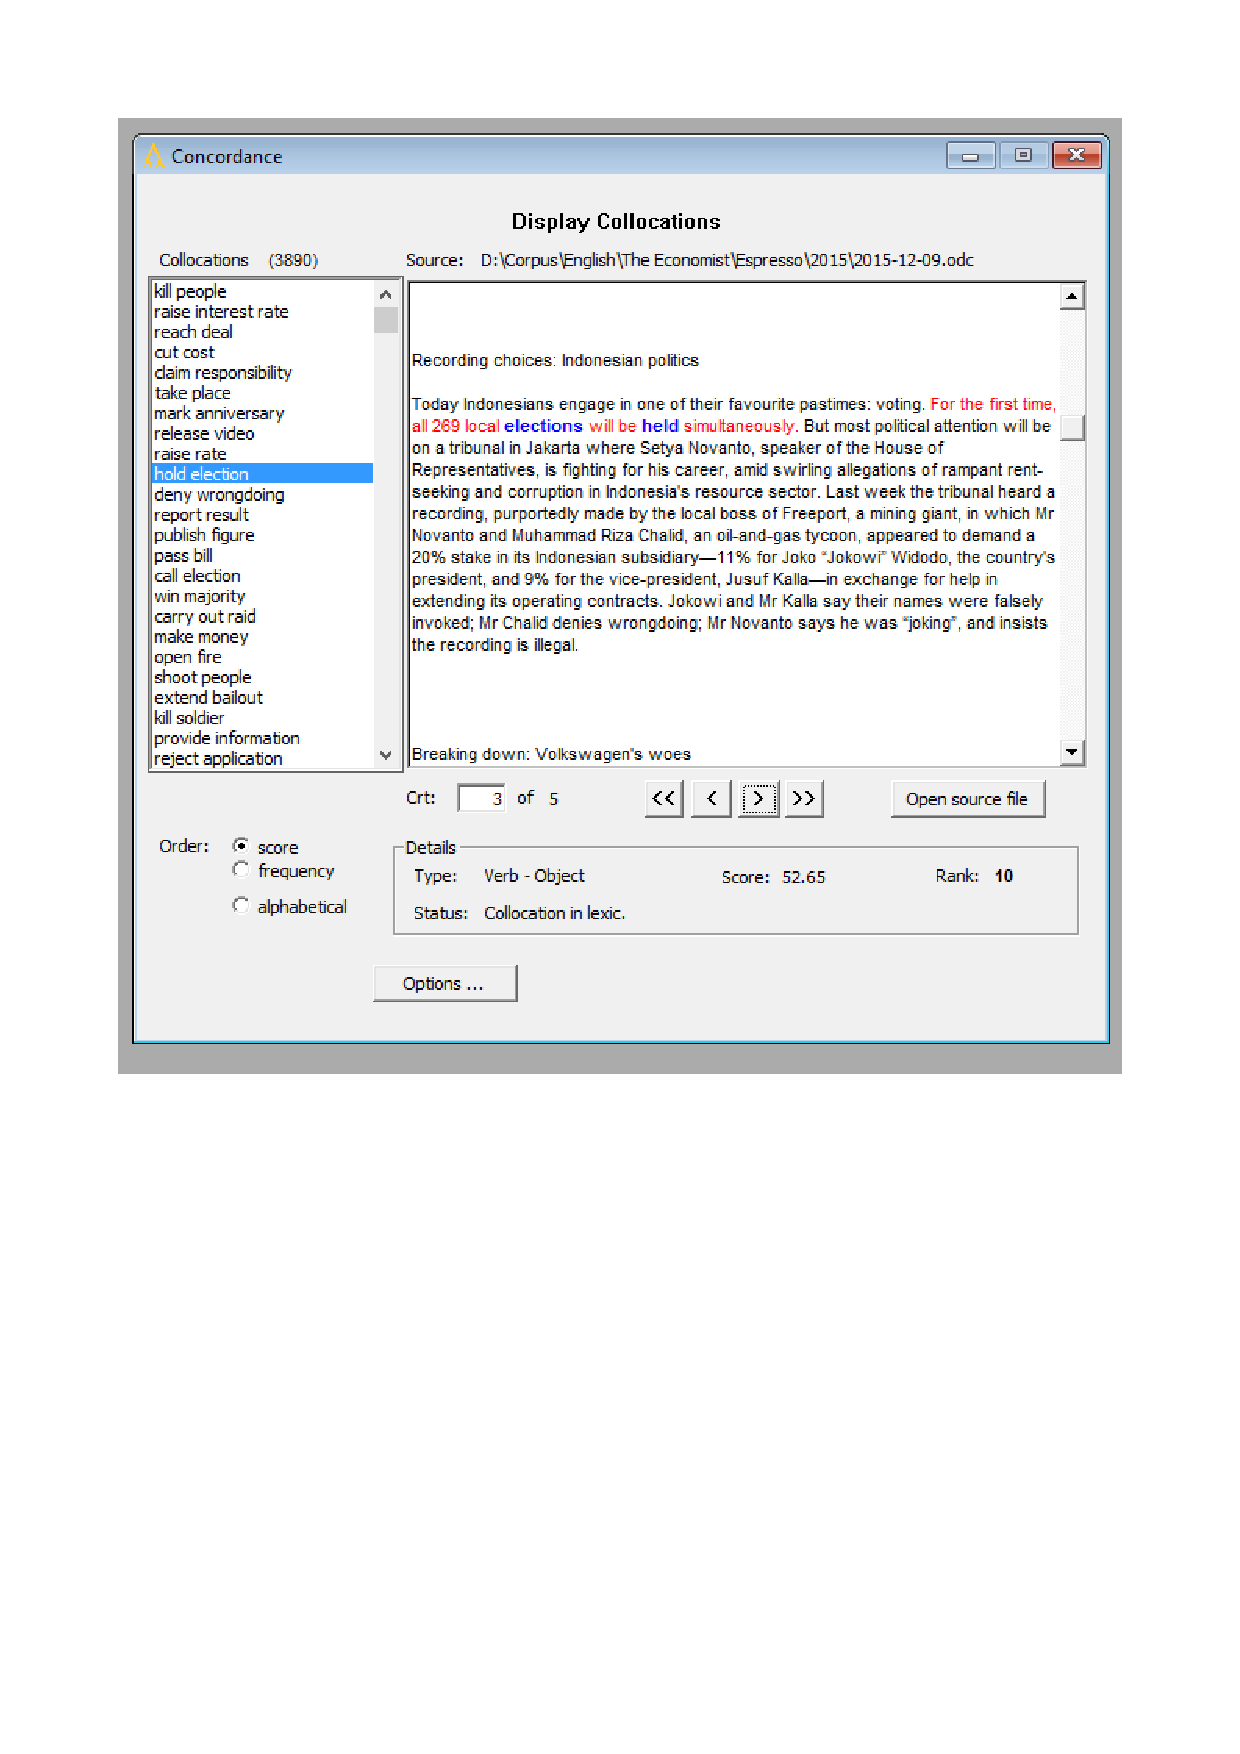
\includegraphics[width=\textwidth, clip=true, trim=0mm 110mm 20mm 10mm]{figures/FipsCoPict.pdf}
%      \includegraphics[width=\textwidth, clip=true, trim=0mm 110mm 20mm 10mm]{figures/FipsCoGUI.pdf}
      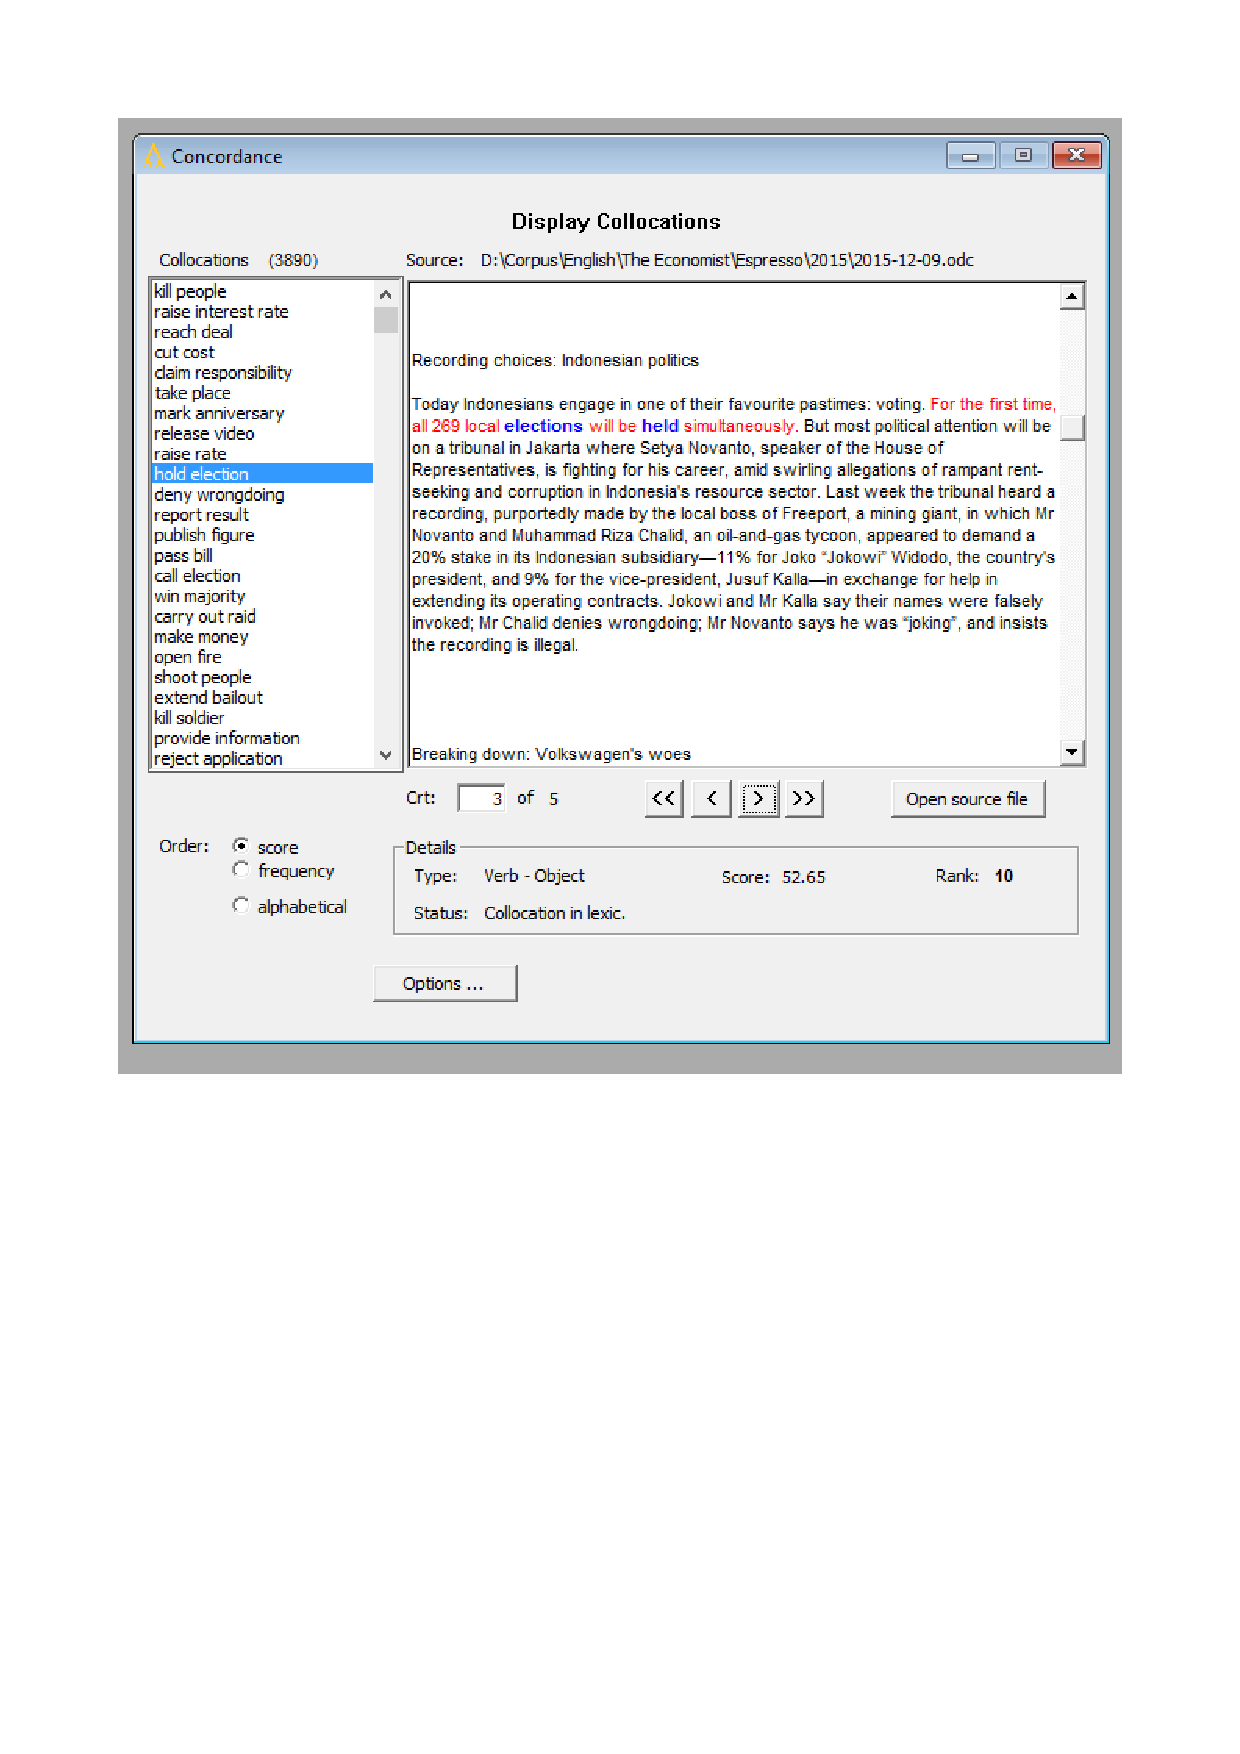
\includegraphics[scale=0.7, clip, trim=20mm 110mm 20mm 20mm]{figures/FipsCoPict.pdf}
%\vspace{-3cm}
\caption{\label{fou:figFips}Extraction of verb-object collocations}
\end{figure}


Figure~\ref{fou:figFips} displays a list of verb-object collocations extracted from an \ili{English} corpus taken from the magazine \textit{The Economist}. On the left, candidate collocations are listed and at the same time they are shown in their context.
          
 
Our system recognizes a large range of collocation types (more than 30 types), including several nominal and verbal ones. The most frequent types are:
\begin{itemize}
\item 	Adjective-noun, e.g. \textit{nuclear war};
\item	Noun-noun, e.g. \textit{flower shop};
\item	Noun-preposition-noun, e.g. \textit{casco di banane} (`bunch of bananas');
\item	Verb-object where the object is a bare noun, e.g. \textit{take part};
\item	Verb-preposition-noun, e.g. \textit{bring to light};
\item	Verb-adverb, e.g. \textit{put together}.
\end{itemize}
\vspace{3mm}

		Once filtered and ordered by means of standard association measures, the candidate collocations are manually validated and added to the lexical database. The current content of the database for six European languages is shown in Table~\ref{fou:fig6}.

\begin{table}[p]
  \begin{tabular}{lrrrrrr}
    \lsptoprule
    collocation type & \ili{English}	& \ili{French} &	\ili{German}	& \ili{Italian}	& \ili{Spanish}	& Greek\\ %\hline
    \midrule
    Adjective-noun	& 3,049	& 5,935 & 	490 &	1,325	& 1,621 & 20,131	\\
    Noun-noun	& 5,671 & 	454 & 	2,476  &	131 &	66	& 471\\
    Noun-prep-noun & 555 & 7,846 & 22 & 1,246 & 988 & 11 \\
    Verb-object	 & 850 &	1,560 &	197 &	250 &	1,098	& 382\\
    Others	& 932 &	2,963 &	330 &	209	 & 592 & 126\\\midrule
    Total	& 11,057	& 18,758 &	3,515 &	3,161 &	4,365	& 21,122 \tabularnewline
    \lspbottomrule
  \end{tabular}
  \caption{\label{fou:fig6}Number and types of collocations in the Fips lexical database}
\end{table}

\section{Evaluation and results}
\label{fou:sec6}
The Fips parser performs well compared to other ``deep'' linguistic parsers (Delph-in,\footnote{International consortium developing HPSG grammars and other tools, cf. \url{http://www.delph-in.net/wiki/index.php/Home}.} ParGram,\footnote{ParGram is an international consortium for the development of LFG-based grammars, see \url{http://pargram.b.uib.no}.} etc.) in terms of speed. Parsing time depends on two main factors: (i) the type and complexity of the corpus, and (ii) the selected beam size (maximum number of alternatives allowed). By default, Fips runs with a beam size of 40 alternatives, which gives it a speed ranging from 150 to 250 tokens (word, punctuation) per second. At that pace, parsing a one million word corpus takes approximately 2--3 hours. We are going to present the experiments that were performed for \ili{Modern Greek} and \ili{English} in order to evaluate the performance of our parser. 

\subsection{Modern Greek}
The evaluation measures the performance of our parser to identify collocations that are lexicalized (i.e. collocations that are present in the lexical database). We also measure the impact of the collocation knowledge on the performance of the parser (in percentage of complete analyses). To achieve the evaluation, we took a small newspaper corpus of about 20,000 words  and we manually identified 638 collocations (both nominal and verbal). We ran the parser twice on the corpus: the first time before and the second time after enrichment of the collocation database. 
On the first run, the parser achieved 43.26\% of complete analyses and identified 124 collocations. On the second run, after enrichment of the lexicon, the percentage of complete analyses increased to 44.33\% and nearly three quarters of the corpus collocations were identified (482/638). Over this small corpus, the parser achieved a 100\% precision in the \isi{collocation identification} task, with a recall of 75.54\% and an F-measure of 86\%. The collocations that were not identified (156 out of 638) were part of sentences for which the parser did not achieve a complete analysis.
	
\subsection{English}
We have also conducted an evaluation over a corpus with approximately 6,000 sentences taken from \textit{The Economist}. The research questions were specifically focused on the statistical significance of ambiguity resolution based on collocation knowledge and on how frequently, in a given corpus, the detection of a collocation helps the parser make the ``right'' decision. 
To answer those questions, we parsed the corpus twice, first with the \isi{collocation detection} component turned on and then with the component turned off. We then compared the results of both runs. Since it was difficult to compare phrase-structure representations, we used the Fips tagger, that is the Fips parser with part-of-speech output. It is indeed much easier to compare POS-tags than phrase-structures. Tables~\ref{fou:fig7} and~\ref{fou:fig8} illustrate the Fips tagger output for the \isi{segment} in boldface of the sentence \textit{The researchers estimated \textbf{the total worldwide labour costs} for the iPad at \$33, of which China’s share was just \$8}.

Table~\ref{fou:fig7} gives the results obtained with the \isi{collocation detection} component turned on, and Table~\ref{fou:fig8} the results obtained with the component turned off.
 
\begin{table}
  \begin{tabular}{>{\itshape}l>{\scshape}lrl}
    \lsptoprule
    \normalfont word & \normalfont tag & position & collocation \\ %\hline
    \midrule
    the       & det & 27\\
    total     & adj & 31 \\
    worldwide & adj & 37 \\
    labour    & noun & 47 \\
    costs & \textbf{noun} & 54 & \itshape labour costs \tabularnewline
    \lspbottomrule
  \end{tabular}
  \caption{\label{fou:fig7}Parser output \textit{with} collocation knowledge}
\end{table} 
 

\begin{table}
  \begin{tabular}{>{\itshape}l>{\scshape}lrl}
    \lsptoprule
    \normalfont word & \normalfont tag & position & collocation \\ %\hline
    \midrule
    the       & det & 27\\
    total     & adj & 31 \\
    worldwide & adj & 37 \\
    labour    & noun & 47 \\
    costs & \textbf{verb} & 54 \tabularnewline
    \lspbottomrule
  \end{tabular}
  \caption{\label{fou:fig8}Parser output \textit{without} collocation knowledge}
\end{table} 
 
 
 

The sentence \isi{segment} \textit{the total worldwide labour costs} is displayed in both tables with the words in the first column, the part-of-speech tag in the second column and the position – expressed as position of the first character of each word starting from the beginning of the sentence – in the third column. As we can see, the word \textit{costs} is taken as a noun in the first analysis, as a verb in the second. The (correct) choice of a nominal reading in the first analysis is due to the detection of the collocation \textit{labour costs}. In the second run, given the absence of collocational knowledge, the parser opts for the verbal reading. Both output files could easily be manually compared using a specific user interface as illustrated in the screenshot in Figure~\ref{fou:figScreen}, where POS differences are displayed in red.

\begin{table}[h]
  \begin{tabular}{lSS}
    \lsptoprule
    & \multicolumn{1}{c}{with collocations} & \multicolumn{1}{c}{without collocations} \\ %\hline
    \midrule
    complete analyses & 73.41\% & 72.95\% \\
    POS-tag differences & 727 \\
    better tags & 382 & 106\\
    number of collocations & 1668 & \multicolumn{1}{c}{-} \tabularnewline
    \lspbottomrule
  \end{tabular}
  \caption{\label{fou:fig9}POS-tagging with and without collocation knowledge\todo[inline]{value missing in row 2, col 3? Please indicate if n/a}}
\end{table}  

\begin{figure}[p]
%\vspace{-4cm}
%\hspace{-10cm}
  %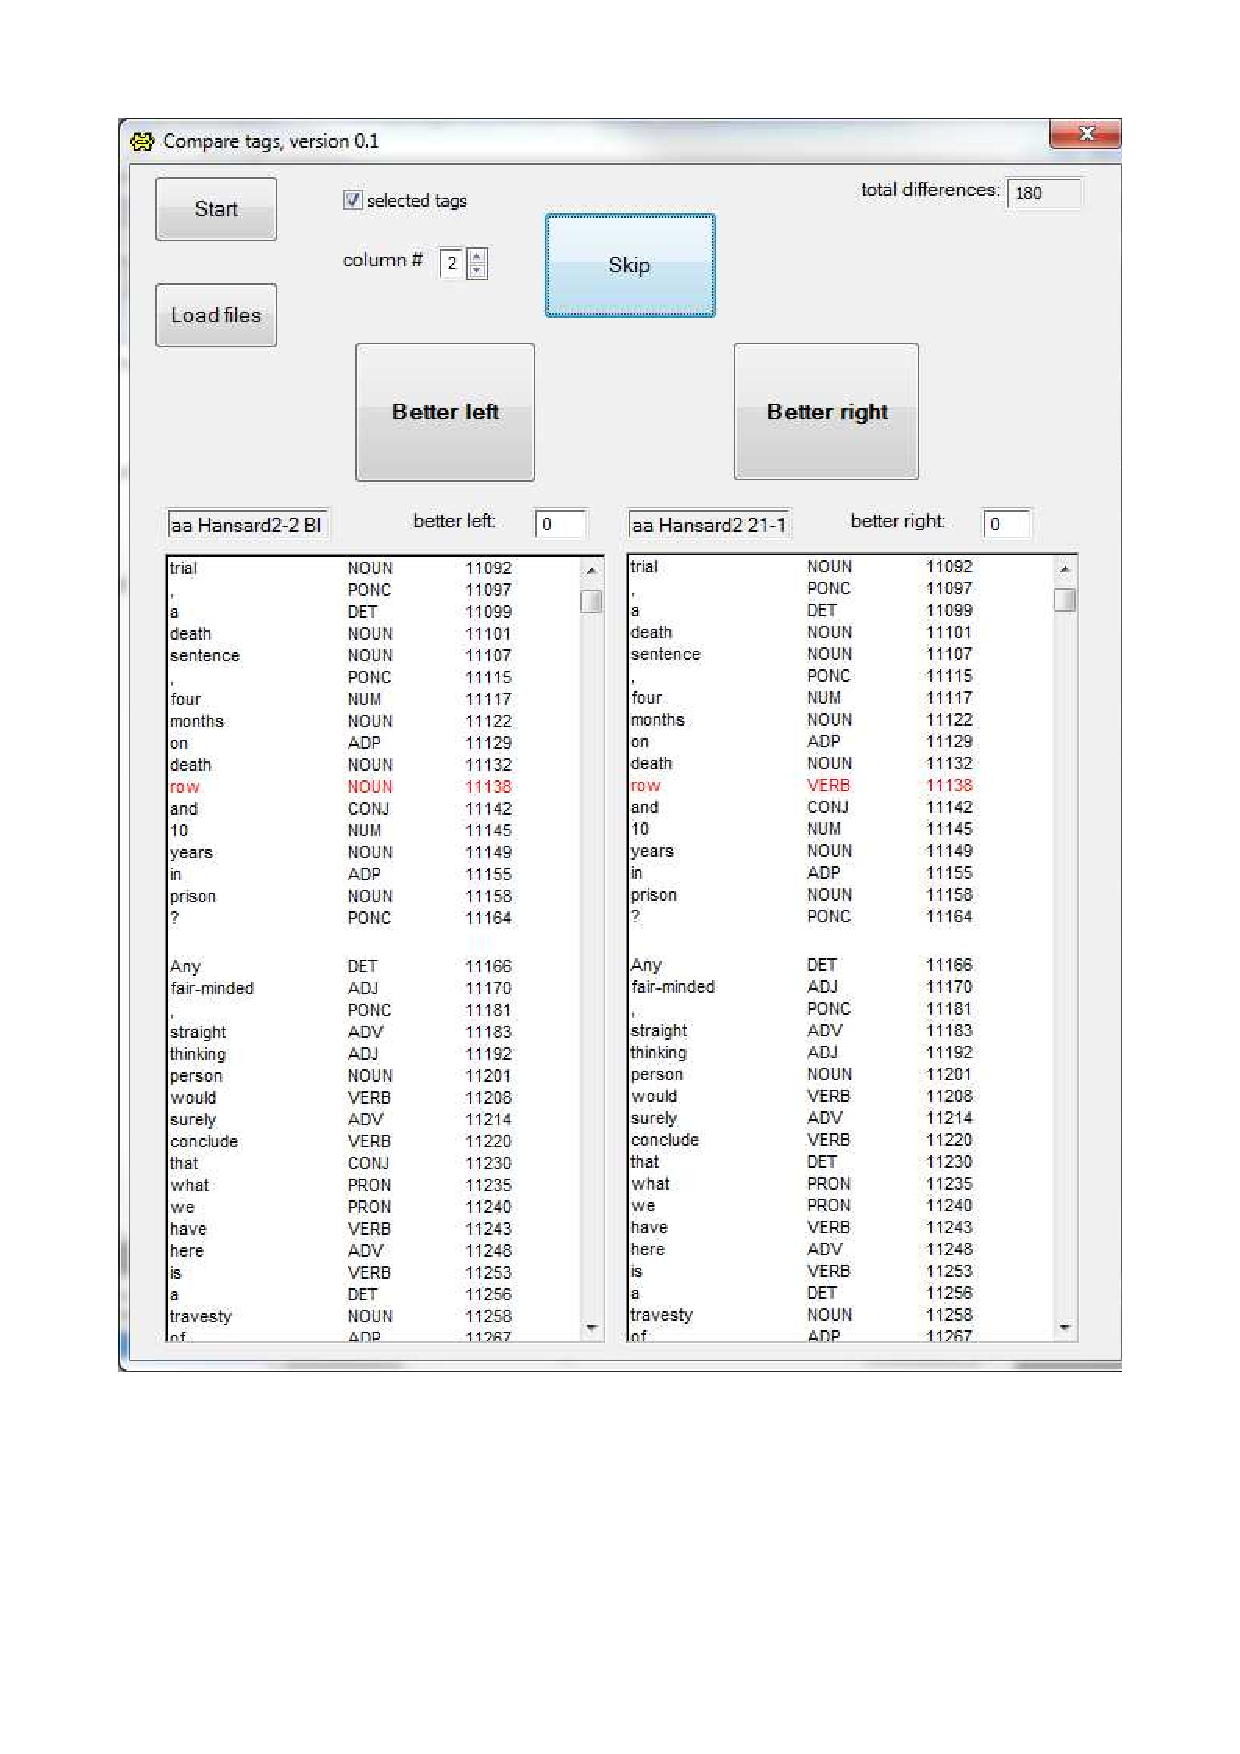
\includegraphics[scale=0.8, clip, trim=20mm 60mm 20mm 20mm] {figures/fips-screenshot.pdf}
  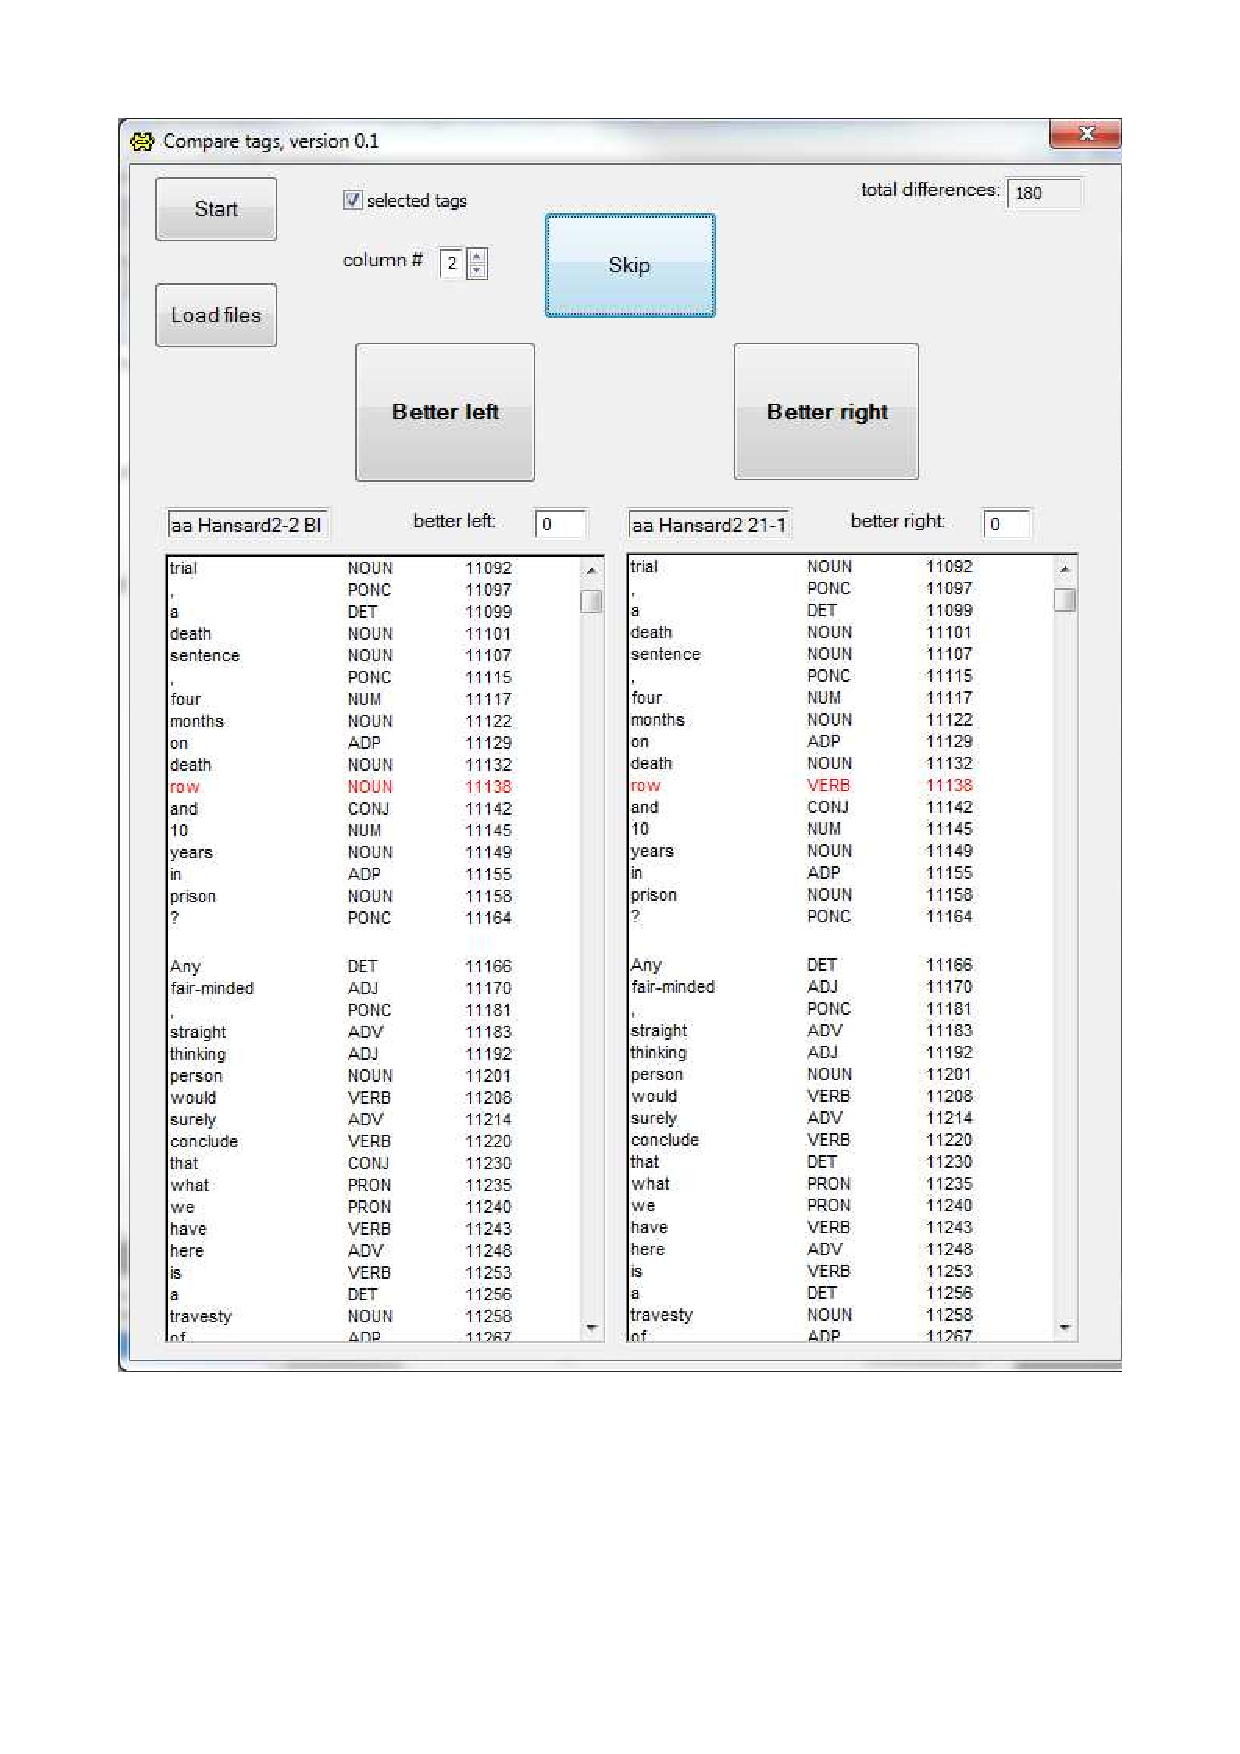
\includegraphics[width=\textwidth, clip, trim=20mm 60mm 20mm 20mm]{figures/fips-screenshot.pdf}
\caption{\label{fou:figScreen}The evaluation user interface}
\end{figure}

A summary of the results of the evaluation is given in Table~\ref{fou:fig9}. The first line shows the number of complete analyses. Collocational knowledge increases the number of complete analysis by approximately 0.5\%, or about 30 sentences for our corpus of 6,000 sentences. 727 tags are different between the two runs. Of those, excluding differences which do not really matter (some words can be analyzed either as predicative adjectives or as adverbs without much semantic differences, etc.), in 382 cases the tags were better in the first run (with collocational knowledge), and 106 cases better in the second run (without collocational knowledge). In other words, collocational knowledge helped the parser make the better decision four times more than it penalized it. Notice finally that 1,668 collocations were detected in the corpus (more than one in four sentences), which clearly stresses the high frequency of this phenomenon in natural language.

\section{Conclusion}
\label{fou:sec7}
In this chapter, we have argued in favour of a treatment of collocations, and by extension of all MWEs, fully integrated in the parsing process. The argument is rather simple. On the one hand, we have shown that the identification of collocations must be based on analyzed data, and therefore cannot be performed before parsing. On the other hand, we have also shown that \isi{collocation identification} can help the parser, for instance to solve lexical as well as syntactic ambiguities, provided that the identification is done before the end of parsing. The solution to this apparent paradox -- \isi{collocation identification} cannot be done before and cannot be done after parsing -- is clear: \isi{collocation identification} must be part of the parsing process and must be performed as early as possible, that is at the time the parser attaches the second constituent of the collocation, or inserts the trace of that constituent. 

%\bibliographystyle{langsci/langscibook}
%\bibliography{lrec2014-admin} 

\section*{Abbreviations}
Tagset from \cite{petrov12}.
\begin{multicols}{2}
\begin{tabbing}
NOUN \hspace{1em} \= coordinating conjunction\kill
    \scshape adj \> adjective \\
    \scshape adp \> adposition \\
    \scshape adv \> adverb \\
    \scshape conj \> coordinating conjunction \\
    \scshape det \> determiner \\
    \scshape noun \> noun \\
    \scshape num \> numeral \\
    \scshape pron \> pronoun \\
    \scshape prt \> particle     \\
    \scshape punc \> punctuation \\
    \scshape verb \> verb \\
    \scshape x \> other
\end{tabbing}
\end{multicols}
%\section*{Acknowledgements}

{\sloppy\printbibliography[heading=subbibliography,notkeyword=this]}
\end{document}
